\documentclass{mcmthesis}
\mcmsetup{CTeX = true,   % 使用 CTeX 套装时,设置为 true
        tcn = 83723, problem = B,
        sheet = true, titleinsheet = true, keywordsinsheet = true,
        titlepage = false, abstract = false}
\usepackage{palatino}
\usepackage{lipsum}
\usepackage{url}
\setlength{\headheight}{13.6pt}
\begin{document}
\title{Precise Prediction, Optimal Selection}
\date{\today}
\begin{abstract}
\hspace*{1mm}In this paper, three models are presented to describe the demographic trend and the geographical distribution of some most populated languages. We take many factors such as culture and migration into consideration and analyse the problem from different perspectives in these models. We establish an additional model using integer programming to figure out the best strategy for the distribution of enterprise offices, which based on AHP analysis of all possible factors.\\
\hspace*{8mm}The first part is based on the fact that the demographic change in language is mainly influenced by the changes in population and migration patterns in the country. We used Logistic, Gaussian and other methods to analyze the data of existing linguistic populations and predict future trends.\\
\hspace*{8mm}In the second part, we use Agent model, which is relatively new, to simulate microcosmic mechanism of communication between different languages and form a conclusion that a language which has higher statue is more likely to become dominant in linguistic population. As the statues of languages are based on many factors such as economy and net migration rate, we take them into account and establish the Markov chain model to predict geographical distribution of some top languages in the future from a macroscopic view.\\
\hspace*{8mm}In the third part,we use AHP method which based on the data of online inquiry survey to figure out the weight ratio of 7 major factors. It could help us to conduct integer programming to find the best strategy of the distribution of enterprise offices. We change the weight ratio and the initial conditions to simulate the reform of communication technology. Five new offices is definitely a better choice according to our simulation. The adjusted choices are also listed.\\
\hspace*{8mm}Finally, in the sensitivity analysis, we also point out the advantages and disadvantages of our model.
\begin{keywords}
Agent model; Markov chain; AHR; Regression analysis;
\end{keywords}
\end{abstract}
\maketitle

\section{Introduction}
\subsection{Background of the problem}
\hspace*{8mm}Language is a system that consists of the development, acquisition, maintenance and use of complex systems of communication, particularly the human ability to do so; and a language is any specific example of such a system [1]. There are currently about 6900 languages spoken on Earth, and half the world's population claim ten major languages as a native language. Furthermore, with the development of economics, travelling efficiency, technology (especially network), globalization and culture shock, more and more people choose some languages as their second language, or even third language. \\
\hspace*{8mm} As an essential part of communication, different language consists different social environment. Moreover, the factors mentioned above is going to have a great impact on our society. We are amazed to find out that academic consensus holds that between 50\% and 90\% of languages spoken at the beginning of the 21st century will probably have become extinct by the year 2100. [1] How will the population of certain languages change in the future? Will the population of a certain language change when a new type of language comes into the environment? What factors should we take into consideration? These questions have lingered in our minds during the contest.

\subsection{Restatement of the problem}
\hspace*{8mm}In our discussion, we find that this place-selecting problem should be applied with a 0-1 model when considering the short-term development of the company, and we should consider several factors to optimize the function to come up with a better suggestion. When it comes to the long-term development of the company, we should consider the change of geographic distribution of language over time to make more profit. Based on the logic order to analyze the problem, we divide the problem into four parts.\\
\begin{itemize}
\item Step 1: Analyze the factors such as migrants, population growth, tourists, and the migration and assimilation of cultural groups that may affect the distribution of language speakers.\\
\item Step 2: Build a simulation model to simulate the language competition in different conditions such as the population, complexity of social network, etc.\\
\item Step 3: Build a regression model to find the change of the distribution of language speakers over time.\\
\item Step 4: Build a 0-1 selection model to find an optimal solution to the company place selection.\\
\end{itemize}

\subsection{Overview of our work}
\hspace*{8mm}After identifying and restating the problem, we use several models to solve our problems.
\begin{itemize}
\item Firstly, we use the official data on World Bank of each country from 1960 to 2015 in a five-year cycle to establish a population-language regression model over time.
\item Secondly, based on the model we make, we draw a graph to demonstrate the change of the population in these languages in the past, to predict the population in the future.
\item Thirdly, we use the Agent Social Circle Network Model of Linguistic Population Change in the Language Change Toolbox in Netlogo to simulate micro language change, and then use the Markov chain to the deal with the macro language change to establish a model for geographic distributions of these languages.
\item Next, we use AHP and 0-1 model and graph theory to predict 6 optimal places for the company and reduce the number of optimal places to save resource and money for the company.
\end{itemize}

\section{Assumptions and Justifications}
\begin{itemize}
\item Assumption: Studying the pattern of population growth on a five-year cycle applies to all languages of the study and can estimate or predict the population of each language on a five-year cycle further.
\item Assumption: We don't consider the impact to the population of the language caused by the total time of work or tour.
\item Justification: According to the footnote in our research data in World Bank. [2] We find out that the best time-cycle to research on population changes is five years, because five years fit in well with a study, or work cycle abroad, and the net migration rate has a leap on a fifteen-year cycle which can be divided by five.
\item Assumption: We don't consider those languages which are endangered, becoming extinct, or developing stably but in a small population. Therefore, based on the linguistic demographic rankings given by Ethnologue[3], we choose these top fifteen languages as our main research objects in this problem.
\item Justification: Although there are many languages in the world, many of them are regarded as endangered, or greatly endangered. Moreover, about half the world's population claim ten major languages as a native language, so we just extend the range to top fifteen languages in case that the top ten will be replaced by other language.
\item Assumption: We don't consider severe environmental changes on the Earth such as asteroid collisions, natural disasters, etc. or huge geographical changes on the Earth such as some lands are submerged by the rise of ocean, etc.
\item Justification: These things are recognized as low-probability things, and we don't need to focus on them.
\item Assumption: The national population growth rate is the same as the population growth rate of the country in various languages.
\item Justification: We assume that the political, economic and education environment are stable in 50 years. Hence, the proportion between national population and native language speakers is approximately a constant. So, the number of native speakers is changing mainly according to the national population.
\item Assumption: The life expectancy of migrants is calculated by normal distribution.
\item Assumption: We consider that people's native language is the same as the native language in the place they are born. (a.k.a. mother tongue)
\item Justification: This is a culture tradition and is accepted by the whole world. Moreover, an migrant's mother tongue after immigration is still the mother tongue in the country, which will have a counter-productive role in processing data and should be taken into consideration.
\end{itemize}

\section{Notations}
\begin{tabular}{c|l}
Variable & Notation \\
\hline $PA$ & migrants in country A who died in year N \\
\hline $QAN$ & the population in country A in year N \\
\hline $MAN$ & the net migrants in country A in year N \\
\hline $WAN$ & the number of people that take a certain language as their native language \\
\hline $UAN$ & the work or travel population in country A in year N \\
\hline $GAN$ & the total number of people that speak a certain language \\
\hline $L(t)$ & Logistic function \\
\hline $G(x)$ & Gaussian interpolation formula \\
\hline $E(x)$ & Exponential interpolation formula \\
\hline $F(x)$ & Fourier interpolation formula \\
\hline $P_x$ & the percentage of language 0 speakers (dominant) \\
\hline $P_y$ & the percentage of language 1 speakers (intruder) \\
\hline $P_z$ & the percentage of language 0\&1 speakers (bilingual) \\
\hline $Prob(x)$ & probability of $x$ \\
\hline $C_{ij}$ & the highest rate circulating from one language $i$ to $j$ \\
\hline $S_x$ & the order of language $x$ in the society \\
\hline $a$ & influence rate between languages \\
\hline $n_i(t)$ & the total number of people using language $i$ by time \\
\hline $Q$ & a quasi-transfer matrix \\
\hline $w_i$ & population out divided by total population of language i \\
\hline $r_i$ & population in divided by total population of language i \\
\hline $R(t)$ & the total population of immigration \\
\hline $W(t)$ & the total population of emigration \\
\hline $\alpha$ & the rate of the total number of people is increasing \\
\hline $\lambda_{max}$ & the maximum eigenvalue of the matrix \\
\hline $C_r$ & the judgment index \\
\hline $c_i$ & the consistency index \\
\hline $r_i$ & the average consistency index data \\
\end{tabular} \\

\section{Models}
\subsection{Model I: A regression model to predict approximate language population change}
\subsubsection{Modeling ideas}
\hspace*{8mm}Based on the official data of each country in a five-year cycle from 1960 to 2015, we estimate the number of national migrants, the number of immigrants from all countries, the population growth in different regions, the migration and assimilation of cultural groups, and political and social environment to establish a language population regression model over time and predict the population-language pattern in 50 years.
\subsubsection{Formulas and notations}
\begin{equation}
PA = \sum(MA(N-t_1)*N(t_1,y))
\end{equation}
In which, \\
$PA$ is migrants in country A who died in year N.
\begin{equation}
WAN = QAN - MAN + PA
\end{equation}
In which, \\
$QAN$ is the population in country A in year N. \\
$MAN$ is the net migrants in country A in year N. \\
$WAN$ is the number of people that take a certain language as their native language. \\
\begin{equation}
GAN = WAN + LAN + UAN 
\end{equation}
In which, \\
$UAN$ is the work or travel population in country A in year N.\\
$GAN$ is the total number of people that speak a certain language.\\

To predict the numbers of MAN, QAN, and UAN, we use logistic method to deal with most of the conditions, and some interpolations such as Gaussian and Exponential interpolations for some "abnormal" countries to make our model more robust. Here are the formulas below.\\
Logistic formula:
\begin{equation}
L(t)=\frac{K}{(1+\frac{K}{N_0}-1)\exp(-rt)}
\end{equation}
Gaussian interpolation formula:
\begin{equation}
G(x)=a_1\exp(-(\frac{x-b_1}{c_1})^2)+a_2\exp(-(\frac{x-b_2}{c_2})^2)+a_3\exp(-(\frac{x-b_3}{c_3})^2)
\end{equation}
Exponential interpolation formula:
\begin{equation}
E(x)=a\exp(bx) + c\exp(dx)
\end{equation}
Fourier interpolation formula:
\begin{equation}
F(x)=a_0+a_1\cos(wx)+b_1\sin(wx)+a_2\cos(wx)+b_2\sin(wx)+a_3\cos(wx)+b_3\sin(wx)
\end{equation}

\subsubsection{Calculations in this model}
\hspace*{8mm}Based on the population and migration data from 1960 to 2015 we get, we use the curve fitting toolbox (a.k.a. cftool) in MATLAB to predict the value of WAN in 50 years. And we will take some "minor" factors such as the migration and assimilation of cultural groups in the sensibility analysis to judge if this model is robust. Here are the prediction pictures we draw with MATLAB. The initial year (year 0) is 1960 because if we use the original years, the graph would be bad.

\begin{figure}[h]
\small
\centering
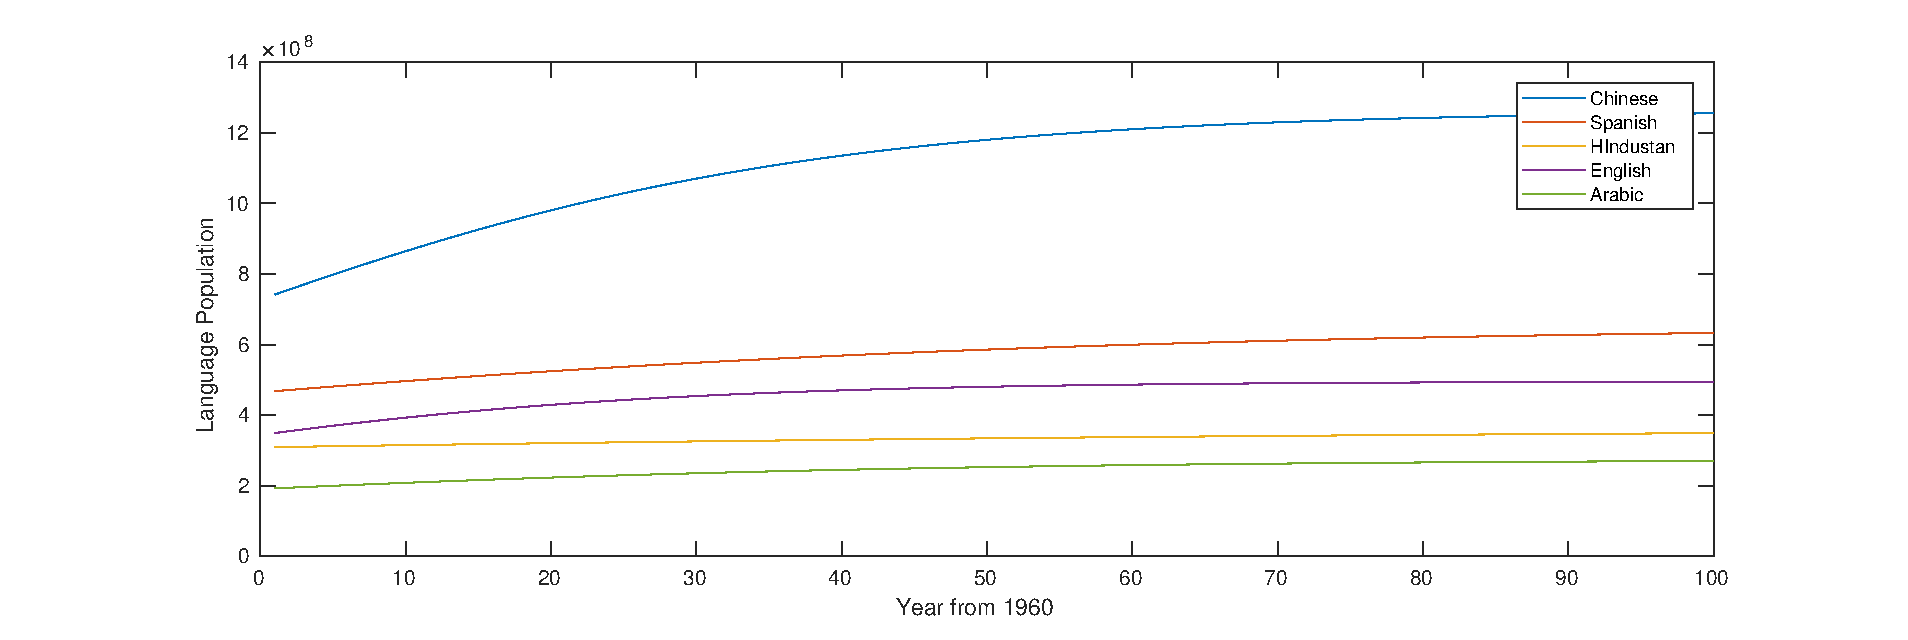
\includegraphics[width=12cm]{picture_1_from_1_5.eps}
\caption{Top 1-5 Language} \label{fig:Top 1-5 Language}
\end{figure}

\begin{figure}[h]
\small
\centering
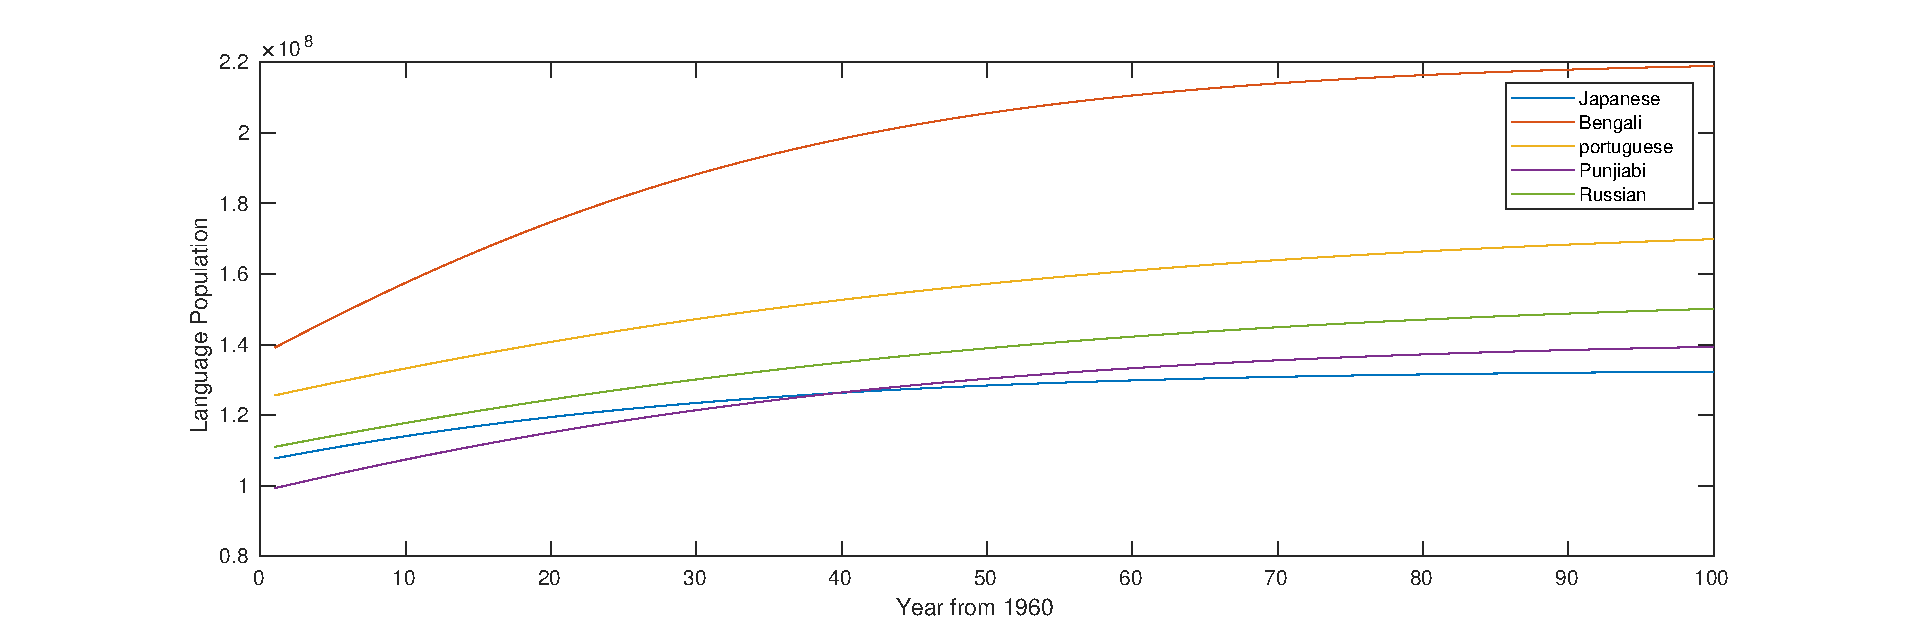
\includegraphics[width=12cm]{picture_2_from_6_10.eps}
\caption{Top 6-10 Language} \label{fig:Top 6-10 Language}
\end{figure}

\subsubsection{Information we can get from our model}
\hspace*{8mm}In our model, we find out that the population of language speakers is heavily based on the population of the country and the migration pattern. \\
\hspace*{8mm}From the image, we can observe that the top-ranked languages will increasingly be used by language learners as a second language due to their large base, large population, broad coverage, and the wave of immigrants brought by globalization and tourism.\\ \hspace*{8mm}Furthermore, more and more speakers take them as a second language and make their population increase stably. The representative languages are English, Mandarin and Hindustani. As for Spanish and Arabic, the growth trend will basically remain unchanged, because they have a large circle of audience.\\
\hspace*{8mm}We classify them as a "Logistic" growth pattern, in which the condition of those languages is mature and stable and will increase stably with the passage of time. However, this increase isn't eternal due to resource restrictions, etc.\\
\hspace*{8mm}It is noteworthy that several lower-ranked languages, such as Russian, and French, has showed strong uncertainty in the curve rankings, such as slowing down or even stagnating in our model. In the future, these top-ten languages are highly likely to be replaced by Japanese, Portuguese, French, and so on. This mainly derives from low birth-rate, unstable political environment which are bad for language growth.\\
\hspace*{8mm}We classify them as a "Gaussian" growth pattern, in which the condition of those languages is not that stable and indicates downside risk in the future. This pattern can be converted to "Logistic" pattern when better environment is provided. Meanwhile, if the environment isn't improved, these languages will face the risk of depression.\\
\hspace*{8mm}These languages, Malay, Hausa and Punjabi, are currently used in large numbers with large population growth rates, which will surpass some countries with lower growth rates in the short term and the total population will rise.\\ 
\hspace*{8mm}However, at the same time, we can see from the statistics that these countries have many migrants. From our perspective, in the coming decades, the migration rate in these countries won't slow down and their output to top five language-speaking countries will continue to grow. Hence, the language population will slowly decrease and may be surpassed by those developed countries such as French, German, and Japanese in the long run.\\
\hspace*{8mm}We classify them as a "Exponential" growth pattern, in which the condition of those languages is prosperous and will prosper in a short time. But as time goes by, their prosperity will be slowly converted to more mature patterns such as a "Logistic" pattern. Furthermore, the prosperity is not so stable that it will be affected by many factors.\\

\subsection{Model II: Agent social circle network model to simulate competition between two languages}

\subsubsection{Modeling ideas}
\hspace*{8mm}On the premise of mastering the data of the trend of global immigration, we use the Agent social circle network model in Netlogo to simulate the micro-language exchange. Agent network model establishes the language communication network in the field of computer simulation, defines the social radius size, sets the language types with different population proportions, increases the birth rate, death rate and migration rate to reproduce the social appearance, and introduces the horizontal and longitudinal communication model to simulate the language competition. [4]In our model, we use the Language Change Toolbox [5] in Netlogo [6] to simulate the micro-language exchange. This model can be the fundamentals towards the geographical distribution of languages.
\subsubsection{Formulas and notations}
\hspace*{8mm}To focus on the most important things such as the colony number, the percentage, the language influence rate, we make this model a bit easier by reducing the variables in the model.\\
$P_x$: the percentage of language 0 speakers(dominant).\\
$P_y$: the percentage of language 1 speakers (intruder).\\
$P_z$: the percentage of language 0\&1 speakers (bilingual).\\
In which, $P_x+P_y+P_z=1$ \\
Vertical model: parent to son:
\begin{eqnarray}
Prob(x-x)=1 \\
Prob(y-y)=1 \\ 
Prob(z-x)=C_{zx} S_x X^a \\
Prob(z-y)=C_{zy} S_x X^a \\
Prob(z-z)=1-Pr(z-x)-Pr(z-y)
\end{eqnarray}
Horizontal model: person to person in one generation
\begin{eqnarray}
Prob(x-x)=1-C_{xz} S_y y^a \\
Prob(x-z)=C_{xz} S_y y^a \\
Prob(y-y)=1-C_{yz} S_x x^a \\
Prob(y-z)=C_{yz} S_x x^a \\
Prob(z-z)=1
\end{eqnarray}
In which, \\
$x-x,y-y,z-z,z-x,z-y$: language circulating from parent to son in vertical model, person to person in one generation in horizontal model.\\
$C_{zx}=C_{zy}, C_{yz}=C_{xz}$: the highest rate circulating from one language to another.\\
$S_x, S_y$: the place of each language in the society, in which $S_x + S_y = 1$. \\
$a$: influence rate between languages.
\subsubsection{Calculations in this model}
\hspace*{8mm}We modify some the code in Netlogo to make it fit. %Here is the picture of the graphical user interface in Netlogo.
Here are the steps of this model.
\begin{itemize}
\item Step 1: Create 1000 agents in a $120\times120$ space.
\item Step 2: Set up the intruder language rate to 5\%(based on net migration rate) and randomly set the distribution of these agents.
\item Step 3: Set up the "reward" mode to simulate migrate pattern.
\item Step 4: Set up the influence rate to adjust the pattern.
\item Step 5: Change the number of agents, intruder language rate, influence rate and repeat Step 2 to Step 4 to see if there are any changes or patterns in the variation.
\end{itemize}

\subsubsection{Information we can get from our model}
\hspace*{8mm}The network model of agent social circle with linguistic and demographic changes is a simulation of the micro-language exchange, which shows the prediction of the living conditions of the small-scale bilingual population under certain conditions and can be extended to the whole world. Here are the results we get.\\

influence rate$=0.025$ 
\begin{tabular}{c|c|c|c|c}
Agents & 5\% & 10\% & 15\% & 20\% \\
100	& 0	& 0	& 0	& 0 \\
200	& 0	& 0	& 0.01 & 0.01 \\
300	& 0	& 0.005	& 0.01 & 0.02 \\
400	& 0	& 0.005	& 0.025	& 0.045 \\
500	& 0	& 0	& 0.05 & 0.055 \\
600	& 0	& 0.01 & 0.05 & 0.06 \\
700	& 0	& 0.01 & 0.05 & 0.08 \\ 
800	& 0.01 & 0.02 & 0.08 & 0.11 \\
900	& 0.01 & 0.05 & 0.12 & 0.17 \\
1000	& 0.01 & 0.06 & 0.12	 & 0.19 \\
\end{tabular} \\ 

influence rate$=0.050$ 
\begin{tabular}{c|c|c|c|c}
Agents & 5\% & 10\% & 15\% & 20\% \\
100	& 0.01	& 0.01	& 0.01	& 0.02 \\
200	& 0.015	& 0.02	& 0.04 & 0.06 \\
300	& 0.04	& 0.04	& 0.08 & 0.18 \\
400	& 0.04	& 0.07	& 0.12	& 0.16 \\
500	& 0.02	& 0.08	& 0.16 & 0.24 \\
600	& 0.04	& 0.08 & 0.19 & 0.37 \\
700	& 0.06	& 0.12 & 0.25 & 0.42 \\ 
800	& 0.07 & 0.20 & 0.24 & 0.75 \\
900	& 0.07 & 0.15 & 0.35 & 0.78 \\
1000	& 0.11 & 0.2 & 0.51	 & 0.87
\end{tabular} \\
From this table we can find that:
\begin{itemize}
\item the larger total people become, the less an intruder language is able to take the place.
\item the larger intruder language become, the more an intruder language is able to set foot on this land.
\item the larger influence rate is, the more an intruder language is able to set foot on this land. 
\item Furthermore, a little bit change on the influence rate will cause great influence on the language distribution.
\end{itemize}
\hspace*{8mm}The world is a complex and complex multilingual system. No matter how we change the initial conditions, the most influential language will further expand the trend in the long run. That's to say, we can predict that Chinese and English will cover most regions of the world in the future and their circles in the long run. Meanwhile, more and more languages which are rarely used will become extinct or greatly endangered.\\

\subsection{Model III: Markov chain model to draw the geographical language patterns}
\subsubsection{Modeling ideas}
\hspace*{8mm}Markov chain model is a stochastic forecasting model, which considers the evolution of the historical state of events, and predicts the trend of future states by calculating the state transition probability. By analyzing the evolution characteristics of population data and historical situation, Markov chain model can be used to establish discrete population prediction model.[7]
\subsubsection{Formulas, notations and calculations}
\hspace*{8mm}Let the world's top 15 most widely used languages be our subjects, Structural changes are the increase, reduction, entry (immigration into the country using those languages), emigration (emigration from the country using those languages). 
\begin{equation}
N(t)=\sum_{i=1}^{15}{n_i(t)}
\end{equation}
In which, \\
$(n_1(t),n_2(t),\cdots,n_{15}(t))$ is the population of each language used during the year of t. \\
$N(t)$ is the total number of people using these languages. \\
\begin{equation}
Q=(q_{ij})_{15\times15}
\end{equation}
In which, \\
$q_{ij}$ is the percentage of the population of $i$ transferred from $i$ to $j$ divided by the population of $i$ every year. \\
$Q$ is a quasi-transfer matrix(the sum of the elements of each row $ \leq 1$). \\
subject to:
\begin{eqnarray}
\sum_{i=1}^{15}{q_{ij}}+w_i=1, \\
r_i \geq 0, \\
\sum_{i=1}^{15}{r_i}=1
\end{eqnarray}
In which, \\
$w_i = {\text{population out from language i}}/{\text{total population of language i}}$, \\
$r_i = {\text{population into language i}}/{\text{total population of language i}}$, \\
\begin{eqnarray}
N(t+1)=N(t)+R(t)-W(t) \\
N_j(t+1)=\sum_{i=1}^{15}{n_i(t) q_{ij}}+r_i R(t)-n_j(t) w_j \\
M(t)=N(t+1)-N(t)=R(t)-W(t)
\end{eqnarray}
In which, \\
$R(t)$ is the total population of immigration. \\
$W(t)$ is the total population of emigration. \\
\begin{equation}
M(t)=\alpha N(t), \alpha=\frac{N(t+1)}{N(t)}-1, a_j(t)=\frac{n_j(t)}{N(t)}
\end{equation}
\begin{eqnarray}
a_j(t+1) = \frac{1}{1+\alpha}[\sum_{i=1}^{15}{a_i{t}(q_{ij}+r_j w_j)}-w_j a_j(t)+\alpha r_j]
\end{eqnarray}
In which, \\
$\alpha$ is the rate of the total number of people is increasing. \\
In particular, when $\alpha = 0$,
\begin{equation}
\alpha_j(t+1)=[\sum_{i=1}^{15}{a_i{t}(q_{ij}+r_j w_j)}-w_j a_j(t)]
\end{equation}
Let $a(t)=(a_1(t),\cdots,a_7(t)), P'=(p'_{ij})$, in which
\begin{equation}
p'_{ij}=
\begin{cases} 
	q_{ij}+r_j w_i, &\text{$i\neq j$}\\
  	q_{ij}+r_j w_j - w_j, &\text{$i=j$}
\end{cases}
\end{equation}
This is the equation that the distribution of the Markov chain with P' as the transfer matrix satisfies at $T$-time.

\subsubsection{Information we can get from our model}
\hspace*{8mm}Using MATLAB program to simulate computation, we can find out the change of language distribution in a period of time with the migration trend and Markov matrix. The simulation is as follows: \\
\begin{figure}[h]
\centering
\includegraphics[width=12cm]{picture_3_2018_language_population.png}
\caption{Language Population in 2018} \label{Language Population in 2018}
\end{figure}
\begin{figure}[h]
\centering
\includegraphics[width=12cm]{picture_4_2060_language_population.png}
\caption{Language Population in 2060} \label{fig:Language Population in 2060}
\end{figure}
Note: Green ones are global agencies location in the following context.

\subsection{Model IV: Use AHP and 0-1 model to select the best place}
\subsubsection{Modeling ideas}
\hspace*{8mm}The establishment of a global office requires consideration of different considerations, including economic development, transport time, transport costs and communication fluency. The objective is to establish 6 specific additional office locations to radiate to all important areas and maximize the overall benefits. First, we use analytic hierarchy process(AHP) to carry on the weight sorts to each influence factor.[8] Next, we use 0-1 integer programming based on graph theory method to decide the best office location.\\
\hspace*{8mm}Analytic Hierarchy Process (AHP): Analytic hierarchy process is a kind of mature algorithm for weight sorting. We establish the assumption and calculation of analytic hierarchy process according to existing rules and circumstances.\\
\hspace*{8mm}0-1 Integer Programming based on Graph Theory: We use integer programming to predict the locations of new offices around the world, based on the weight ratios of various factors. In this section, for the accuracy of the results, we have taken about 35 major locations around the world to compare them and to determine the best eight locations (including existing New York and Shanghai Agencies) through integer programming.

\subsubsection{Formulas and notations}
First, we define a vector $V=\{v_1,v_2,v_3,v_4,v_5,v_6,v_7\}$ \\
In which,\\

\begin{tabular}{c|l}
Name & Description \\
\hline $v_1$ & regional economic development \\
$v_2$ & traffic time \\
$v_3$ & transportation costs \\
$v_4$ & education level \\
$v_5$ & political stability \\
$v_6$ & language communication mobility \\
$v_7$ & climate conditions \\
\end{tabular} \\
$a_{ij}$ is the ratio of $x_i$ and $x_j$ to measure a factor's influence.\\
Obviously, $a_{ji}={1}/{a_{ij}}$ \\
And we use the well-known psychological scale by Satty, in which: \\

\begin{tabular}{c|l}
Scale & Definition \\
\hline
1 & To represent the same importance with two factors \\ 
3 & The former is slightly more important than the latter. \\
5 & The former is relatively more important than the latter. \\
7 & The former is significantly more important than the latter. \\ 
2, 4, 6, 8 & Represents the average of the adjacent judgments above. \\
\end{tabular} \\
$C_r$ is the judgment index, and $C_r=c_i / r_i$. \\
In which, \\
$\lambda_{max}$ is the maximum eigenvalue of the matrix. \\
$c_i$ is the consistency index, and $c_i=\lambda_{max}-7/(7-1)$. \\
$r_i$ is the average consistency index data in the 7 order matrix. \\
The optimization function for each country:
\begin{equation}
Z_i=\sum_{1\leq j \leq7}{P_{x_{i_j}} A_j}
\end{equation}
In which, \\
$P_{x_{i_1}}-P_{x_{i_7}}$ is the seven indicators of a country based on flashback world rankings.

\subsubsection{Calculations in this model}
\hspace*{8mm}Firstly, we list the vectors that affect the factor. From the psychological point of view, too much grading can surpass people's judgment ability, increase the difficulty of making judgment, and provide false data easily. Some researchers have also used experimental methods to compare the correctness of people's judgment results under various scales, and the experimental results show that the 1-9 scale is the most suitable one.\\
\hspace*{8mm}Secondly, we have conducted a simple random sampling survey for the employees and managers of multinational corporations to obtain the data, construct the matrix after obtaining the $a_{ij}$ data, and then check the consistency of the data using MATLAB.  \\
\hspace*{8mm}Thirdly, we judge the index, and calculate the weight of 7 factors. We get the vector $V=\{0.53,0.19, 0.08, 0.03, 0.05, 0.06, 0.06\}$ and here is a bar chart demonstrating the vector visually.\\
\begin{figure}[h]
\centering
\includegraphics[width=12cm]{picture_5_bar.png}
\caption{Bar Chart} \label{fig:Bar Chart}
\end{figure} \\
\hspace*{8mm}Next, for the accuracy of the results, we have chosen 35 major locations around the world to compare them and to determine the best eight locations (including New York and Shanghai Agencies) through 0-1 integer programming. These places are: \hspace*{8mm}
\begin{tabular}{c|l}
Number & Regions \\
\hline 5 & North America \\
4 & South America \\
4 & Central Europe \\
4 & Southwest/Southern Europe \\
6 & Middle East of North Africa \\
4 & West Asia \\
5 & Northeast Asia \\
3 & South Asia/Oceania \\
\end{tabular} \\
\hspace*{8mm}Then, we will mark these countries from $x_1$ to $x_{35}$ and establish the initial constraint condition of integer programming.
\begin{eqnarray}
x_1+x_2+x_3+x_4+x_5\leq 1 \\
x_6+x_7+x_8+x_9\leq 1 \\
x_{10}+x_{11}+x_{12}+x_{13}\leq 1 \\
x_{14}+x_{15}+x_{16}+x_{17}\leq 1 \\
x_{18}+x_{19}+x_{20}+x_{21}+x_{22}+x_{23}\leq 1 \\
x_{24}+x_{25}+x_{26}+x_{27}\leq 1 \\
x_{28}+x_{29}+x_{30}+x_{31}+x_{32}\leq 1 \\
x_{33}+x_{34}+x_{35}\leq 1
\end{eqnarray} \\
\hspace*{8mm}Next, we base our knowledge on graph theory, combined with the world's air, train, car and other means of transport data to determine the traffic time and transportation costs of the country rankings, and then according to the world's GDP rankings, environmental Protection Agency data, etc. to determine the ranking of other indicators. To make the results more convincing, we chose the top 163 in the rankings, the original 35 candidate countries ranked seven indicators as tables. All rankings are in flashback rankings, IE (163-positive rankings) to facilitate the following calculations. \\
\hspace*{8mm}Finally, by calculation, we get the optimal places. Meanwhile, we review the procedure to see if we can save resource by reducing some of the agencies.

\subsubsection{Information we can get from our model}
\hspace*{8mm}The optimal result is $x_2=x_6=x_{12}=x_{15}=x_{19}=x_{25}=x_{29}=x_{35}=1$. The rest of $x_i=0$. Which means the optimum places are:
\begin{itemize}
\item \textbf{Hong Kong, China} (Cantonese, Mandarin Chinese and English), 
\item \textbf{Mumbai, India} (Hindi, English, Punjabi and Bengali), 
\item \textbf{Cairo, Egypt} (Arabic and English), 
\item \textbf{Madrid, Spain} (Spanish, English and Arabic), 
\item \textbf{Frankfurt, Germany} (German, English and Russian), 
\item \textbf{Rio de Janeiro, Brazil} (Spanish, Portuguese and English).
\end{itemize}
\hspace*{8mm}From what we can find, although this is a short-term forecast, these countries or regions are the leading countries in the language region (not necessarily the leading countries of the actual group of countries), and the financial forecasters have positive expectations for their economic development, and there will be no significant change in the political situation. Therefore, the international rankings of their indicators will not fluctuate greatly.\\
\hspace*{8mm}Considering the continuous development of 5G technologies and other communication technology, we suggest that the client company should reduce the number of new international offices to 5 or less for the following reasons:
\begin{itemize}
\item The significant change of global communication will affect our decision in two aspects: the weight ratio of each index of AHP model will obviously change, which is reflected in the increase of the proportion of the economy and the decrease of proportion of traffic time and cost. Other unpredictable changes will also emerge.
\item The new communication technology revolution will influence different countries to varying degrees, so the national rankings of indicators will change, especially the economic indicator. 
\end{itemize}
\hspace*{8mm}To make new decisions, the data we need are listed: the situation of global political change, the development of the communication technology degree in various countries, the new AHP statistics and the global climate change situation, etc. \\
\hspace*{8mm}To simulate, we first assume that the countries' rank unchanged (8 candidate countries or regions have stable economic forecast). The AHP weight ratio is adjusted, initially adjusted to $V'=\{0.61, 0.11, 0.07, 0.04, 0.05, 0.06, 0.06\}$, next we will merge any of the two large language regions and, with Lingo recalculation of the maximum $Z$, and multiply the proportional coefficient u=8/7, compared with the previous data, the results show that after merging southwest Europe, and southern Europe and the Arab region, there will be a certain increase in $Z$ value, indicating that the establishment of 5 new offices is a better choice. We then carried out simulation to repartition Europe and the Middle East countries. We set our target to 7 countries and got different results. The 5 additional offices were:
\begin{itemize}
\item \textbf{Hong Kong, China};
\item \textbf{Mumbai, India};
\item \textbf{Rome, Italy};
\item \textbf{London, the United Kingdom};
\item \textbf{Rio de Janeiro, Brazil}.
\end{itemize}
\hspace*{8mm}We have got an apparent increase in Z, and these countries have relatively better economic expectations, a more stable political structure and a technological revolution facilitating their economic development. With Lingo calculation, the Z value after processing is significantly higher. So if considering the improvement of communication technology, choosing to add these 5 cities as the new offices' address will be a better choice for this global company.

\section{Sensitivity Analysis}
\subsection{Sensitivity analysis of various population models}
The logistic model is stable and has little influence on the population change when the parameter change is 1\%, whereas the exponential model is not stable enough. The model obtained has a great impact on population change when the parameter is reduced by 1\%, and eventually turns to the logistic model.  Gaussian model is special because it is used to describe the population reduction. It has a certain effect on population change when the parameter is increased by 1\%, and it will develop toward logistic model. In contrast, when the parameter is reduced by 1\%, it has little effect on the population change. Considering the sensitivity analysis of the Markov chain, when other factors such as climate have great influence, the model will show great instability.
\subsection{Sensitivity analysis of Agent model in NetLogo}
In reward mode, there exists a sensitivity problem of language favorability. When alpha values are raised from 0.05 to 0.1, even only 5\% of foreign languages can affect the local language ratio, creating a 1:1 coexistence system. However, when alpha values vary from 0.05 to 0.025 or from 0.1 to 0.2, the effect on the final state is relatively small. Therefore, the language favorability will obviously affect the language competitive relationship.
\subsection{Sensitivity analysis of AHR-0-1 model}
The economy is always dominant and the economic impact is the greatest. Despite this, with the development of society, technology will make up for the disadvantage of distance, and the cultural exchange between countries has become a factor influencing company's development; that is to say, countries that are  technology-driven as well as with significant cultural diversity benefit company's development in the long run.

\section{Strengths and Weaknesses}

\subsection{Strengths}
\begin{itemize}
\item The main strength of our model is close to the reality. The demographic trend and immigration trend is considered when we analyse the growth of language population.
\item The language-population model we make (Model I) can describe better than original logistic models and is more robust.
\item To make the model more convincing, we study the patterns of language distribution both in microscopic view (by Agent model) and macroscopic view (by Markov chain).
\item Besides, by considering 7 factors, we improve the model to let it predict the best place for new corporation offices more precisely.
\item In order to predict situations in the future, we change the initial conditions many times to simulate the possible circumstance of global development and have a definite answer.
\end{itemize}

\subsection{Weaknesses}
\begin{itemize}
\item The calculation of our model is complex, we need to find the most suitable regression model for each major language.
\item When predicting the distribution of language population in the future, we didn't take factors such as climate and political change into consideration. Hence, we can't figure out a precise prediction.
\item Our AHP analyse are not very precise because we have limited time and resource to do the survey.
\end{itemize}

\section{A Memo}
To: Chief Operating Officer of the company \\
From: Team 83723 \\
Date: February 13th, 2018 \\
Subject: Results and recommendations on location options \\

At your request, we have recently conducted a survey on global trends about language to provide you with a solution for your new office location. Using data from the World Bank's total population and the number of net migrations of all countries from 1960 to date as well as the 2015 version \textit{Ethnologue} , we have created a demographic model that reflects the use of languages over time, and analyzed the top-ranked language.\\
\hspace*{8mm}Utilizing common demographic mathematical methods, we find that:\\\hspace*{8mm}\textbf{English, Mandarin Chinese and Hindustani, languages that ranked top as the most widely-used, will continue to accelerate their growth rate whether in the short term or in the long term.} This obvious conclusion can be validated by the following reasons: 
\begin{itemize}
\item(1) The base of the usage in each language is large;
\item(2) Some giant countries that mainly use these languages (the United States, China, and India) have tremendous economic strength;
\item(3) As a result of (2) and national policies to promote the influx of migrants in these countries further increase the population; 
\item(4) More and more language learners use them as a second language. These facts are applied mathematically in the model.
\end{itemize}
\hspace*{8mm}\textbf{Spanish and Arabic will continue to grow at a small rate in the future, whose growth trends are basically consistent with the current ones.} The advantages of these two languages lie in the wide range of population, covering different continents, and having long-term value in the context of economic integration and the Internet. The disadvantage lies in the unstable political environment of some local regions, which may have potential unknown negative effects on economic and technological development. \\
\hspace*{8mm}\textbf{Russian, Malay and French, ranked 6 to 10, whose growth trends are very uncertain, show their slow growth rate. There will be even growth stagnation in the future. }As a result of the economic slowdown, there has been a marked rise in low fertility or departures in the corresponding countries. The statuses of these languages are highly likely to be overtaken by those of the languages that are ranked behind them in the near future, such as Japanese, Portuguese and French.\\
\hspace*{8mm}\textbf{Malay, Hausa and Punjabi all have a high rate of population growth, which in the short term will surpass those having low growth rates, with the population rising. In the long run, the number of people who use these languages will decline.} According to the statistics, currently the population using such languages is huge, and similarly the number of new users is large, but the countries where these languages are used are also large immigrant exporters. Addition, the trend is that, in the coming decades, the country's emigration rate will not slow down as locals continue to immigrate to the top five of the language population. Hence in the long run the growth rate of population using the language will slow down and be overtaken by the languages used in developed countries (German, Japanese and Italian etc).\\
\hspace*{8mm}We then selected 35 major global points for agencies, whose positions have been ranked in combination with data from transportation and GDP rankings etc. Apart from New York and Shanghai, we have added 6 new offices (in parentheses are the languages required for the corresponding staff): 
\begin{itemize}
\item \textbf{Hong Kong, China} (Cantonese, Mandarin Chinese and English), 
\item \textbf{Mumbai, India} (Hindi, English, Punjabi and Bengali), 
\item \textbf{Cairo, Egypt} (Arabic and English), 
\item \textbf{Madrid, Spain} (Spanish, English and Arabic), 
\item \textbf{Frankfurt, Germany} (German, English and Russian), 
\item \textbf{Rio de Janeiro, Brazil} (Spanish, Portuguese and English).
\end{itemize}
These 6 locations are optimistic about economic development and the political situation will not change too much. So they are the best choices for the global agencies, both in the long term and in the short term.\\
\hspace*{8mm}Of course, in view of the continuous development of 5G technology and communication technology, the proportion of time consumption on transportation and costs are reduced, and the new evolution communication technology will be different in each country. We have done our best to help you save resources after using our investigation to meet the needs, and in the light of the statistical data on the development of the communications revolution in countries, we find that these new 5 offices are better decisions. The five addresses are: \textbf{Hong Kong, Mumbai, London, Rome, and Rio de Janeiro.} The economic expectations of these regions are relatively better; the political structures are more stable. Plus the scientific and technological revolution can be developed in a better social environment.\\
\hspace*{8mm}We hope that your company can apply the conclusion based on our research and analysis, to select the proper agencies, and hire staff we have recommended.
\newpage
\begin{thebibliography}{99}
\bibitem{1} Language. (2018, January 31). In Wikipedia, The Free Encyclopedia. Retrieved 18:17, February 12, 2018, from \url{https://en.wikipedia.org/w/index.php?title=Language&oldid=823276986}
\bibitem{2} World Bank Open Data. Retrieved 18:50, February 12, 2018, from \url{https://data.worldbank.org/} 
\bibitem{3} "Summary by language size". Ethnologue. Retrieved 12:35 2018-02-09, from \url{https://www.ethnologue.com/statistics/size}
\bibitem{4} A Modeling and Simulation Method for Three Language Competition Models Based on Agent Social Circle Network.(2015) CN Patent App. CN 201,510,244,355. Retrieved 14:59 2018-02-10, from \url{http://www.google.nr/patents/CN104881574A?cl=fr}
\bibitem{5} Troutman, C. and Wilensky, U. (2007). NetLogo Language Change model. \url{http://ccl.northwestern.edu/netlogo/models/LanguageChange}. Center for Connected Learning and Computer-Based Modeling, Northwestern University, Evanston, IL.
\bibitem{6} Wilensky, U. (1999). NetLogo. \url{http://ccl.northwestern.edu/netlogo/}. Center for Connected Learning and Computer-Based Modeling, Northwestern University, Evanston, IL.
\bibitem{7} J. Pan, A. Nagurney (1994). Using Markov chains to model human migration in a network equilibrium framework. Mathematical and Computer Modelling, ISSN: 0895-7177, Vol: 19, Issue: 11, Page: 31-39,
\bibitem{8} Jia QiYuan, Xie JinXing, Ye Jun (2011). Mathematical Model. High Education Press, ISBN: 978-7-04-031150-1, Page: 249-255,
\bibitem{9} M. Garraffa, M. Obregon, A. Sorace (2017) Linguistic and Cognitive Effects of
Bilingualism with Regional Minority Languages: A Study of Sardinian-Italian Adult Speakers. Frontiers in Psychology. November 2017, Volume 8, Article 1907,
\end{thebibliography}

\end{document}
